
\section{代数几何的函子观点}

代数几何中的函子观点将概形视为某种特殊的函子 $\mathsf {Ring}\to\mathsf {Set}$, 也即 ``环范畴上的变集合''. (此处的环是指交换环.) 对于环 $A$, 一个概形的 ``$A$-点'' 即是这个函子在阶段 $A$ 的元素. 一个概形可理解为同时在所有环上解一个方程组, 例如 Fermat 概形为函子 $$A\mapsto \{(x,y,z)\in A^3\mid x^n+y^n=z^n\},$$ 它在阶段 $\mathbb{R}$ 当然有点, 而人们关心的是其在阶段 $\mathbb{Q}$ 是否就有点.

Ingo Blechschmidt 的博士论文 \cite{ILAG} 指出, 在函子观点下, 我们考虑的对象生活在一个\topos{}中, 这个\topos{}的内语言即可用于对这些对象进行各种操作与推理.

\begin{definition}
	[label={affine-line}]
	{(仿射直线与仿射空间, 函子定义)}
	定义\emph{仿射直线} (affine line) $\mathbb A^1$ 为遗忘函子
	$$
	\mathbb A^1\colon \mathsf {Ring}\to\mathsf {Set},A\mapsto A.
	$$
	换言之, 仿射直线的 $A$-点等同于 $A$ 的元素.
	对于自然数 $n$, 定义\emph{仿射空间} $\mathbb A^n$ 为 $(\mathbb A^1)^n$, 即函子 $A\mapsto A^n$. (回忆函子范畴中的极限是逐对象的.)
\end{definition}

%\todo{层语义}

%定义 \ref{affine-line} 表明对任何环 $A$, 仿射直线的 $A$-点等同于 $A$ 的元素.

由于 $\mathbb A^1$ 是环范畴到集合范畴的遗忘函子, 它自然带有一个环结构. 因此在内语言中我们可以像操作一个普通的环一样操作 $\mathbb A^1$.
例如, 对任何整系数多项式 $f\in\mathbb{Z}[x]$, 有多项式映射 $f\colon \mathbb A^1\to\mathbb A^1$.

\begin{example}
	{(多项式方程的解)}
	设 $f\in\mathbb{Z}[x]$ 为整系数多项式. $f$ 在 $\mathbb{A}^1$ 上的 ``解集''
	$$
	\{x\in\mathbb A^1\mid f(x)=0\}
	$$
	为函子
	$$
	\mathsf {Ring}\to\mathsf {Set}, A\mapsto\{x\in A\mid f(x)=0\}.
	$$
	这是因为它按定义是如下的拉回, 而拉回是逐对象计算的.
	% https://q.uiver.app/#q=WzAsNCxbMSwwLCIxIl0sWzAsMSwiXFxtYXRoYmIgQV4xIl0sWzEsMSwiXFxtYXRoYmIgQV4xIl0sWzAsMCwiXFxoc3BhY2V7LTJlbX1cXHt4XFxpblxcbWF0aGJiIEFeMVxcbWlkIGYoeCk9MFxcfSJdLFswLDIsIjAiXSxbMSwyLCJmIiwyXSxbMywxXSxbMywwXV0=
	\[\begin{tikzcd}[ampersand replacement=\&]
		{\hspace{-2em}\{x\in\mathbb A^1\mid f(x)=0\}} \& 1 \\
		{\mathbb A^1} \& {\mathbb A^1}
		\arrow[from=1-1, to=1-2]
		\arrow[from=1-1, to=2-1]
		\arrow["0", from=1-2, to=2-2]
		\arrow["f"', from=2-1, to=2-2]
	\end{tikzcd}\]
	
	一般地, 设 $f_1,\cdots,f_m\in\mathbb{Z}[x_1,\cdots,x_n]$ 为整系数多项式, 其 ``解集''
	$$
	\{x=(x_1,\cdots,x_n)\in\mathbb A^n\mid f_1(x)=\cdots=f_m(x)=0\}
	$$
	为函子
	$$
	\mathsf {Ring}\to\mathsf {Set}, A\mapsto\{x=(x_1,\cdots,x_n)\in A^n \mid f_1(x)=\cdots = f_m(x)=0\}.
	$$
\end{example}

使用含 $\lor,\Rightarrow,\exists$ 等逻辑符号的公式可以定义更多对象. 如下将所谓\emph{乘法群概形}定义为 $\mathbb A^1$ 的一个子集.

%加法和乘法 $+,{\cdot}\colon \mathbb A^1\times\mathbb A^1\to \mathbb A^1$, 零元和幺元 $0,1\colon {*} \to \mathbb A^1$.

%
%\begin{example}
%	{($\mathbb A^1$ 到自身的映射)}
%	态射 $\mathbb A^1\to\mathbb A^1$
%\end{example}

\begin{definition}
	{(乘法群概形, 内语言定义)}
	乘法群概形 $\mathbb G_m$ 是 $\mathbb A^1$ 中的 ``可逆元构成的子集'':
	$$
	\mathbb G_m := \{x\in \mathbb A^1\mid\internalprop{\text{$x$ 可逆}}\}= \{x\in \mathbb A^1\mid \exists y\in \mathbb A^1\,xy=1\}.
	$$
	
	一般地, 群概形 $GL_n$ 是 $(\mathbb A^1)^{n\times n}$ 中可逆矩阵构成的子集:
	$$
	\begin{aligned}
		GL_n &:= \{M\in (\mathbb A^1)^{n\times n}\mid \internalprop{\text{$M$ 可逆}}\}\\&= \{M\in (\mathbb A^1)^{n\times n}\mid \exists N\in (\mathbb A^1)^{n\times n}\,MN=NM=1\}.
	\end{aligned}
	$$
\end{definition}

由定义, $\mathbb G_m$ 是 $\{(x,y)\in\mathbb A^1\times\mathbb A^1\mid xy=1\}$ 在第一分量投影下的像, 故 $\mathbb G_m$ 作为函子可具体表示为
$$
\mathbb G_m\colon \mathsf {Ring}\to\mathsf {Set},\,
A\mapsto \{x\in A\mid \text{$x$ 可逆}\}.
$$

\begin{prop}
	{($\mathbb A^1$ 是 ``域'')}
	$\mathbb A^1$ 是一个 ``域''. 这句话的意思是如下公式成立,
	$$
	\forall x\in \mathbb A^1\, \big( x\neq 0\Rightarrow\internalprop{\text{$x$ 可逆}}\big).
	$$
	(回忆 $x\neq 0$ 是指 $\neg (x=0)$, 即 $(x=0)\Rightarrow\bot$.) 因此, ``乘法群概形'' $\mathbb G_m$ 也可表示为
	$$
	\mathbb G_m = \{x\in\mathbb A^1\mid x\neq 0\}.
	$$
\end{prop}
%\todo{层语义}

\begin{proof}
	
	由层语义 (定义 \ref{sheaf-semantics-inductive}),
	对于 $x_0\in \mathbb A^1(A)=A$, $A\forces (x_0\neq 0)$ 的含义是对任意环同态 $\varphi\colon A\to B$, 若 $\varphi(x_0)=0$, 则 $B=0$ (零环).
	令 $B=A/(x_0)$, 考虑投影映射 $\varphi \colon A\to B$, 得 $B=0$, 即 $(x_0)$ 是 $A$ 的单位理想, $x_0$ 在 $A$ 中可逆.
	
%	只需证明
%	\begin{itemize}
%%		\item 对任意环 $A$ 以及 $x_0\in A$,
%%		$A\forces \big(x_0\neq 0\Rightarrow\internalprop{\text{$x_0$ 可逆}}\big)$.
%%		\item 对任意环 $A$, $x_0\in A$ 以及 $\varphi\colon A\to B$, 若 $B\forces \varphi(x_0)\neq 0,$ 则 $B\forces \internalprop{\text{$\varphi(x_0)$ 可逆}}$.
%	\item 对任意环 $A$, 以及 $x_0\in A$, 若 $A\forces (x_0\neq 0),$ 则 $A\forces \internalprop{\text{$x_0$ 可逆}}$.
%	\end{itemize}
\end{proof}

%\todo{仿射概形在哪里讲}

\begin{definition}
	{(射影空间, 内语言定义)}
	射影空间 $\mathbb P^n$ 是 $\mathbb A^{n+1}$ 中 ``过原点的直线的集合'':
	$$
	\begin{aligned}
		\mathbb P^n&:=
		\{(x_0,\cdots,x_n)\in \mathbb A^{n+1}\mid
		x_0\neq 0\lor\cdots\lor x_n\neq 0\}\big/ \sim,
	\end{aligned}
	$$
	其中 $\sim$ 是如下等价关系.
	$$
	x\sim x'\quad\text{当且仅当}\quad \exists \lambda \in \mathbb G_m\,x'=\lambda x.
	$$
	%由此定义, 要将 $\mathbb P^n$ 写成函子有些困难.
%	可以证明 $\mathbb P^n$ 作为函子 $\mathsf {Ring}\to\mathsf {Set}$ 同构于
%	$$
%	A\mapsto\{
%	
%	\}
%	$$
\end{definition}

\begin{definition}
	{(仿射概形, 函子定义)}
	定义\emph{仿射概形}为可表函子 $\mathsf {Ring}\to\mathsf {Set}$. 对于环 $A$, 记
	$$
	\operatorname{Spec}A = \operatorname{Hom}(A,-)\colon \mathsf {Ring}\to \mathsf {Set}.
	$$
	由米田引理, 仿射概形的范畴 $\mathsf {Aff}$ 等价于 $\mathsf {Ring}^{\op}$.
\end{definition}
\begin{example}
	{}
	\begin{itemize}
		\item 仿射直线 $\mathbb A^1$ 是仿射概形 $\operatorname{Spec}\mathbb{Z}[x]$; 这是因为 环同态 $\mathbb{Z}[x]\to A$ 一一对应于 $A$ 的元素.
		\item 仿射概形的和, 积均为仿射概形: $\operatorname{Spec}A+\operatorname{Spec}B\simeq \operatorname{Spec}(A\times B)$, $\operatorname{Spec}A\times\operatorname{Spec}B\simeq\operatorname{Spec}(A\otimes B)$.
	\end{itemize}
\end{example}

\subsection{``小'' \topos{}与 ``大'' \topos{}}




\section{综合微分几何与光滑无穷小分析}

代数几何的函子观点可类似地用于微分几何.

\subsection{综合微分几何的理论}

我们首先在本小节叙述一种偏向语法的, ``公理化'' 的理论, 而暂时不关心其模型. 我们将看到这种理论的语法比通常的微分几何更加符合直观.

\begin{axiom}
	{(空间)}
	综合微分几何所谓的\emph{空间} (或称\emph{集合}) 是一个固定的\topos{} $\mathcal E$ 中的对象; \emph{光滑映射} (或称\emph{映射}) 是 $\mathcal E$ 中的态射.
\end{axiom}

\begin{axiom}
	{(直线)}
	综合微分几何所谓的\emph{直线}是 $\mathcal E$ 中一个固定的环 $R$.
\end{axiom}

\begin{remark}
	{}
	字母 $R$ 提示了这个对象与通常微分几何的对象 $\mathbb{R}$ 在直观上的相似性, 但它与 $\mathbb{R}$ 有不同的性质, 如 ``幂零无穷小量'' 的存在性. 因此, 我们不能要求 $R$ 是域.
\end{remark}

\begin{definition}
	{(直线上原点的一阶无穷小邻域)}
	定义 $R$ 上 ``原点的一阶无穷小邻域''
	$$
	D = \{x \in R \mid x^2 = 0\}.
	$$
\end{definition}

\begin{example}
	{(相切曲线的共同切向量)}
	平面 $R^2$ 上的直线 $y=0$ 与圆 $x^2 + (y-1)^2 = 1$ 的交集是 $D$. 这是因为将 $y=0$ 代入圆的方程, 就得到 $x^2 + 1 = 1$, 也即 $x^2 = 0$.
	
	\begin{center}
		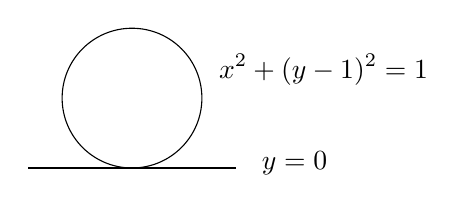
\begin{tikzpicture}[x=0.75pt,y=0.75pt,yscale=-1,xscale=1]
			%uncomment if require: \path (0,300); %set diagram left start at 0, and has height of 300
			
			%Straight Lines [id:da9022525264933119] 
			\draw    (44,106) -- (144,106) ;
			%Shape: Circle [id:dp5620106547865036] 
			\draw   (60.33,72.33) .. controls (60.33,53.74) and (75.41,38.67) .. (94,38.67) .. controls (112.59,38.67) and (127.67,53.74) .. (127.67,72.33) .. controls (127.67,90.93) and (112.59,106) .. (94,106) .. controls (75.41,106) and (60.33,90.93) .. (60.33,72.33) -- cycle ;
			
			% Text Node
			\draw (155.33,97) node [anchor=north west][inner sep=0.75pt]   [align=left] {$\displaystyle y=0$};
			% Text Node
			\draw (134.67,50) node [anchor=north west][inner sep=0.75pt]   [align=left] {$\displaystyle x^{2} +( y-1)^{2} =1$};
		\end{tikzpicture}
	\end{center}
	
	直观上, 直线与圆相切, 两者在相切处有一条公共的 ``无穷小线段''. 更一般地, 任意两条相切的曲线都有一条公共的形如 $D$ 的无穷小线段, 这便是两条曲线共同的切向量.
\end{example}

\paragraph{Kock--Lawvere 公理与导数}

~

\begin{axiom}
	[label={Kock--Lawvere-D}]
	{(Kock--Lawvere 公理)}
	对任意映射 $f \colon D \to R$, 存在唯一的 $a,b\in R$,
	使得
	$$
	f(d) = a + d\cdot b,\quad\forall d\in D.
	$$
	换言之, 作为 $R$-代数有
	$$
	\operatorname{Hom}(D,R) \simeq R[x]/(x^2).
	$$
\end{axiom}

Kock--Lawvere 公理反映了如下的直观: $R$ 上的一个函数在一个很小的邻域上近乎是一次函数.
由此, 我们立刻得到如下的推论.

\begin{propdef}
	{(导函数)}
	对任意函数 $f\colon R\to R$, 存在唯一的函数 $f' \colon R \to R$ 满足
	$$
	f(x+d) = f(x) + d \cdot f'(x),\quad \forall x\in R\,\forall d\in D.
	$$
	称 $f'$ 为 $f$ 的\emph{导函数}. 归纳地定义 $k$ 阶导数 $f^{(k)}(x)$.
\end{propdef}

也就是说, 综合微分几何要求任何函数 $R\to R$ 都是任意次可导的.

\paragraph{Weil 代数与无穷小几何对象}

~

无穷小线段 $D$ 对应代数 $R[x]/(x^2)$. 一般地, 在代数--几何对偶中与无穷小几何对象相对应的代数是 $R$ 上的 \emph{Weil 代数}\footnote{Weil 代数有两种含义, 这里所说的不是来自 Lie 代数的那种 Weil 代数.}.
\begin{definition}
	[label={SDG-Weil-algebra}]
	{(Weil 代数)}
	Weil 代数是形如 $W = R \oplus J$ 的 $R$-代数,
	其中 $J$ 是有限生成自由 $R$-模,
	且为幂零理想. 等价地,
	$$
	W = R[x_1,\cdots,x_n]/I,
	$$
	且存在正整数 $N$ 使得 $x_i^N \in I\,(i=1,\cdots,n)$.
\end{definition}

\begin{remark}
	{}
	上面的概念在 ``经典数学'' (经典逻辑) 中对应\emph{局部 Artin 代数}, 其中 Artin 代数是指不存在无限的理想下降链 (这称为\emph{下降链条件}) 的代数.
	设 $k$ 为域, $A$ 是局部 Artin $k$-代数, $\mathfrak m$ 是 $A$ 的唯一极大理想, 并且额外假设 $k \to A/\mathfrak m$ 是同构.%其剩余域 (residue field).
	可以证明\footnotemark $A \simeq k\oplus\mathfrak m$, $\mathfrak m$ 是有限维 $k$-线性空间且为幂零理想. 定义 \ref{SDG-Weil-algebra} 即是这个结果的类比.
	
	局部 Artin 环在代数几何的形变理论中有重要作用, 这正是因为它对应无穷小几何对象.
\end{remark}

\footnotetext{由中山 (Nakayama) 引理以及下降链条件可得 $\mathfrak m$ 幂零; 又由下降链条件可得每个 $\mathfrak m^j / \mathfrak m^{j+1}$ 是有限维 $k$-线性空间, 从而 $A$ 是有限维 $k$-线性空间.}

\begin{definition}
	{(Weil 代数的谱)}
	对于 Weil 代数 $W$, 定义 $W$ 的\emph{谱}为 $R$-代数同态的空间
	$$
	\operatorname{Spec}W = \operatorname{Hom}_{R\mathsf {Alg}}(W,R),
	$$
	称之为\emph{无穷小几何对象}.
\end{definition}

\begin{example}
	{(常见的无穷小几何对象)}
	\begin{itemize}
		\item 点 $$\text{pt} \simeq \{x\in R\mid x=0\} = \operatorname{Spec} R;$$
		\item 无穷小线段的平方 $$D^2 \simeq \{(x,y)\in R^2 \mid x^2=y^2=0\} = \operatorname{Spec}R[x,y]/(x^2,y^2);$$
		\item $R^2$ 上原点的一阶无穷小邻域 $$D(2) := \{(x,y)\in R^2\mid x^2=xy=y^2=0\} = \operatorname{Spec}R[x,y]/(x^2,xy,y^2);$$
		\item 高阶无穷小邻域
		$$
		D_k := \{x\in R\mid x^{k+1}=0\} = \operatorname{Spec}R[x]/(x^{k+1})\, (k=1,2,3,\cdots).
		$$
	\end{itemize}
\end{example}

前面介绍的 Kock--Lawvere 公理可表述为 $\operatorname{Hom}(\operatorname{Spec}R[x]/(x^2),R) \simeq R[x]/(x^2)$. 类似地有如下公理.

\begin{axiom}
	{(Kock--Lawvere 公理)}
	对于 Weil 代数 $W$, 有
	$$
	\operatorname{Hom}(\operatorname{Spec}W,R)\simeq W.
	$$
\end{axiom}

\begin{remark}
	{(Weil 代数与 Kock--Lawvere 公理的直观)}
	设 $W=R\oplus J$ 是 Weil 代数. 投影 $W \to R$ 对应点 $\text{pt}$ 到无穷小几何对象 $\operatorname{Spec}W$ 的\emph{原点}的嵌入 $$\text{pt} = \operatorname{Spec} R \to \operatorname{Spec}W.$$
	Kock--Lawvere 公理说的是 Weil 代数 $W$ 等同于 $\operatorname{Spec}W$ 上的函数代数. 投影 $W\to R$ 可视为 $\operatorname{Spec}W$ 上的函数在原点处取值; 理想 $J$ 是投影 $W\to R$ 的核, 可视为在原点取值为 $0$ 的函数的集合.
	要求 $J$ 为\emph{幂零}理想, 也即要求在原点取值为 $0$ 的函数都幂零, 直观上说明 $\operatorname{Spec}W$ 是 ``无穷小'' 的.
\end{remark}

Lawvere 以如下的性质刻画无穷小几何对象.

\begin{definition}
	{(无穷小对象, 奇妙右伴随)}
	对于空间 $S$, 若 $(-)^S$ 有右伴随, 则称 $S$ 为\emph{无穷小对象}. 记该右伴随为 $(-)_S$, 称之为\emph{奇妙右伴随} (amazing right adjoint).
\end{definition}

\begin{example}
	{}
	在集合范畴 $\mathsf {Set}$ 中, 只有终对象 $1$ 是无穷小对象.
\end{example}

\begin{remark}
	[label={infinitesimal-object-intuition}]
	{}
	回忆对\topos{}中任意对象 $S$, $(-)^S$ 都有左伴随 $(-)\times S$, 而 $(-)^S$ 有右伴随是非常稀奇的事情. 重要的是此时 $(-)^S$ \emph{保持余极限}. 一个直观如下. 设空间 $X$ 被一族空间 $U_i$ 覆盖 ($X$ 可写成 $U_i$ 和 $U_i\times_X U_j$ 的某种余极限), 那么 $X^S$ 也被 $U_i^S$ 覆盖, 即 $S$ 到 $X$ 的任何映射都必须穿过某个 $U_i$; 这是 $S$ 的像 ``太小'' 导致的.
	
	类似的性质在不是\topos{}的范畴中也有用处. 例如 Abel 群范畴 $\mathsf {Ab}$ 中, 函子 $\operatorname{Hom}(A,{-})$ 保持余极限当且仅当 $A$ 是有限生成投射 $\mathbb{Z}$-模, 这也是一种 ``小'' 的性质.
	
	%映射 $X^D \to Y$ 等同于映射 $X \to Y_D$
\end{remark}

\todo{使用 SDG 的例子, 如 Riemann 曲率}

\todo{无穷小对象的定义, amazing right adjoint}

\subsection{综合微分几何的模型}

本小节介绍综合微分几何的一些模型. 相对简单的模型就能实现 Kock--Lawvere 公理; 而为了使模型满足更多的公理, 以及更加贴近传统的微分几何 (更加 ``有用''), 我们就需要作越来越复杂的调整.
构造综合微分几何模型的贯穿始终的思想是\emph{代数--几何对偶}.

\subsubsection{``代数'' 模型}

首先考虑一个最简单的模型.
\begin{definition}
	[label={SDG-algebraic-model}]
	{}
	考虑有限表现仿射 $\mathbb{R}$-概形范畴 $\mathbb{R}\mathsf{Alg}_{\text{fp}}^\op$.
	回忆, 有限表现 $\mathbb{R}$-代数即形如 $\mathbb{R}[x_1,\cdots,x_n]/(f_1,\cdots,f_m)$ 的代数; 对于有限表现 $\mathbb{R}$-代数 $A$, 以 $\operatorname{Spec} A$ 表示其在对偶范畴中的化身.
	
	所谓\emph{代数模型} (algebraic model) 是 $\mathbb{R}\mathsf{Alg}_{\text{fp}}^\op$ 上的层\topos{} $$\mathsf {Fun}(\mathbb{R}\mathsf{Alg}_{\text{fp}},\mathsf {Set}).$$
\end{definition}

\begin{definition}
	{(直线)}
	定义 \emph{直线}
	$$
		R
		:=\yo(\operatorname{Spec}\mathbb{R}[x]).
	$$
\end{definition}

\begin{remark}
	{}
	这里考虑的\topos{}是 $\mathbb{R}$-代数的\emph{分类\topos{}}, 而 $R$ 是其中的\emph{一般 $\mathbb{R}$-代数} (generic $\mathbb{R}$-algebra).
	
	这些结论对有限生成 $\mathbb{R}$-代数范畴同样成立.
\end{remark}

注意到对 $A\in\mathbb{R}\mathsf {Alg}_{\text{fp}}$,
$$
R(A)=\operatorname{Hom}_{\mathbb{R}\mathsf{Alg}_{\text{fp}}^\op}(\operatorname{Spec}A,\operatorname{Spec}\mathbb{R}[x]) = \operatorname{Hom}_{\mathbb{R}\mathsf {Alg}_{\text{fp}}}(\mathbb{R}[x],A) \simeq A\text{ (作为集合)},
$$
我们发现, $R$ 正是代数范畴到集合范畴的遗忘函子
$$
R\simeq \text{遗忘}
\colon \mathbb{R}\mathsf{Alg}_{\text{fp}} \to \mathsf {Set}.
$$
因此, 使用米田方法, 我们就得到
\begin{prop}
	{}
	$R$ 是交换环.
\end{prop}

有了 $R$, 我们考虑 ``由方程定义的子流形''
$$
M = \{(x_1,\cdots,x_n)\in R^n\mid f_1=\cdots=f_m=0\},
$$
其中 $f_1,\cdots,f_m\in \mathbb{R}[x_1,\cdots,x_n]$ 是多项式. 其范畴语义为拉回
% https://q.uiver.app/#q=WzAsNCxbMSwxLCJSXm0iXSxbMCwxLCJSXm4iXSxbMSwwLCIwIl0sWzAsMCwiTSJdLFsxLDAsIihmXzEsXFxjZG90cyxmX20pIiwyXSxbMywxXSxbMywyXSxbMiwwXV0=
\[\begin{tikzcd}[ampersand replacement=\&]
	M \& 0 \\
	{R^n} \& {R^m,}
	\arrow["{(f_1,\cdots,f_m)}"', from=2-1, to=2-2]
	\arrow[from=1-1, to=2-1]
	\arrow[from=1-1, to=1-2]
	\arrow[from=1-2, to=2-2]
\end{tikzcd}\]
对应 $\mathbb{R}\mathsf {Alg}$ 中的推出
% https://q.uiver.app/#q=WzAsNCxbMSwxLCJcXG1hdGhiYntSfVt5XzEsXFxjZG90cyx5X21dIl0sWzAsMSwiXFxtYXRoYmJ7Un1beF8xLFxcY2RvdHMseF9uXSJdLFsxLDAsIlxcbWF0aGJie1J9Il0sWzAsMCwiTSJdLFswLDEsIihmXzEsXFxjZG90cyxmX20pIl0sWzEsM10sWzIsM10sWzAsMl1d
\[\begin{tikzcd}[ampersand replacement=\&]
	? \& {\mathbb{R}} \\
	{\mathbb{R}[x_1,\cdots,x_n]} \& {\mathbb{R}[y_1,\cdots,y_m],}
	\arrow["{y_i\mapsto f_i}", from=2-2, to=2-1]
	\arrow[from=2-1, to=1-1]
	\arrow[from=1-2, to=1-1]
	\arrow[from=2-2, to=1-2]
\end{tikzcd}\]
故
$$
M = \yo(\operatorname{Spec}\mathbb{R}[x_1,\cdots,x_n]/(f_1,\cdots,f_m)).
$$

\begin{definition}
	{(直线上原点的一阶无穷小邻域)}
	定义
	$$
	D := \{x\in R\mid x^2=0\} =  \yo\big({\operatorname{Spec}\mathbb{R}[x]/(x^2)}\big).
	$$
\end{definition}

我们验证它满足公理 \ref{Kock--Lawvere-D}, 以外部语言叙述即
\begin{prop}
	{}
	$$
	R^D(A) \simeq  A[x]/(x^2).
	$$
\end{prop}

\begin{proof}
	由预层\topos{}指数对象的构造 (命题 \ref{presheaf-category-exponential} 的证明),
	\begin{align*}
		R^D(A) &= \operatorname{Hom}(\yo(\operatorname{Spec}A)\times D,R)\\
		&\simeq \operatorname{Hom}\big(\yo(\operatorname{Spec}A)\times\yo(\operatorname{Spec}\mathbb{R}[x]/(x^2)),
		\yo(\operatorname{Spec}\mathbb{R}[x])\big)\\
		&\simeq \operatorname{Hom}\big(\yo(\operatorname{Spec}A\times\operatorname{Spec}\mathbb{R}[x]/(x^2)),
		\yo(\operatorname{Spec}\mathbb{R}[x])\big)\\
		&\simeq\operatorname{Hom}_{\mathbb{R}\mathsf{Alg}}(\mathbb{R}[x],A\otimes \mathbb{R}[x]/(x^2))\\
		&\simeq A\otimes \mathbb{R}[x]/(x^2))\simeq A[x]/(x^2) \text{ (作为集合).}
	\end{align*}
	其中用到 $\mathbb{R}$-代数的张量积是 $\mathbb{R}\mathsf{Alg}$ 中的和, 即 $\mathbb{R}\mathsf{Alg}^\op$ 中的积.%; 而 $\yo(A)\times\yo(B) \simeq \yo(A\times B)$.
\end{proof}





\subsubsection{光滑代数}

$\mathbb{R}$-代数上的运算是多项式运算; 若将多项式运算扩充为全体 ``光滑'' 运算, 则可产生一个更接近微分几何的模型.

\begin{definition}
	{(光滑代数)}
	\emph{光滑代数} ($C^\infty$-代数) 是指满足如下条件的集合 $A$: 对每个非负整数 $n$ 与每个 $n$ 元光滑函数 $f\in C^\infty (\mathbb{R}^n,\mathbb{R})$ 都有一个 $n$ 元运算, 称为\emph{光滑运算} $A(f)\colon A^n\to A$,
	使得 $f\mapsto A(f)$ 保持复合, 即对于 $h = g \circ (f_1,\cdots,f_k)$, 有
	$$A(h) = A(g) \circ (A(f_1),\cdots,A(f_k)).$$ 换言之, 光滑代数是 Lawvere 理论 $\mathsf {CartSp}$ 的模型 (例 \ref{Lawvere-theory-CartSp}). 光滑代数的同态是保持所有光滑运算的映射. 记光滑代数的范畴为 $C^\infty\mathsf{Alg}$.
\end{definition}

\begin{remark}
	[label={remark-smooth-algebra-R-algebra}]
	{}
	如上定义的 $C^\infty$-代数首先是 $\mathbb{R}$-代数: 考虑 $0$ 元函数 $\mathbb{R}^0\to \mathbb{R}$ 就得到了常量 $A^0\to A$,
	考虑加法与乘法函数 $+,\times\colon \mathbb{R}^2\to \mathbb{R}$ 就得到 $A$ 上的加法与乘法, 考虑映射 $\mathbb{R}^3\to \mathbb{R}, (x,y,z)\mapsto x(y+z) = xy+xz$, 使用 $f\mapsto A(f)$ 保持复合的条件, 就得到 $A$ 上的分配律, 如此这般.
\end{remark}

\begin{example}
	{}
	设 $M$ 是光滑流形, 那么 $M$ 上的光滑函数空间 $C^\infty (M)$ 构成光滑代数: 对 $f\in C^\infty (\mathbb{R}^n,\mathbb{R})$, 定义 $A(f)(f_1,\cdots,f_n)=f\circ (f_1,\cdots,f_n)$.
\end{example}

\begin{example}
	{}
	$\mathbb{R}[\varepsilon]/(\varepsilon^2)$ 是光滑代数: 对 $f\in C^\infty (\mathbb{R}^n,\mathbb{R})$, 定义 $$
	A(f)(a_1+b_1 \varepsilon,\cdots,a_n+b_n \varepsilon)
	=f(a_1,\cdots,a_n)
	+\sum_i \frac{\partial f}{\partial x_i}\Big|_{(a_1,\cdots,a_n)} b_i \varepsilon.$$
	$\mathbb{R}[\varepsilon]/(\varepsilon^2)$ 可视为 ``无穷小线段上的光滑函数空间''.
\end{example}

\begin{example}
	{}
	光滑流形上一点处的光滑函数芽 (定义 \ref{germ-and-stalk}) 构成光滑代数.
\end{example}

%\todo{使用一般 Lawvere 代数中有限生成的概念}
%我们需要有限生成 $C^\infty$-代数的概念.
类比于 $\mathbb{R}[x_1,\cdots,x_n]$ 是 $n$ 个元素生成的自由 $\mathbb{R}$-代数 (交换含幺代数), 有如下命题.

\begin{prop}
	[label={freely-generated-smooth-algebra}]
	{}
	$C^\infty (\mathbb{R}^n)$ 是 $n$ 个元素生成的\emph{自由光滑代数}.
\end{prop}

\begin{proof}
	要证明的是对任意光滑代数 $A$ 与任意 $n$ 个元素 $a_1,\cdots,a_n \in A$,
	存在唯一的同态 $\varphi\colon C^\infty (\mathbb{R}^n) \to A$ 将每个坐标函数 $x_i$ 映射到 $a_i$.
	由定义, 对任意 $f\in C^\infty (\mathbb{R}^n)$,
	$\varphi$ 必须把 $f = f\circ (x_1,\cdots,x_n)$ 映射到 $f(a_1,\cdots,a_n)$, 这便唯一确定了 $\varphi$; 而它确实将投影 $x_i$ 映射到 $a_i$: $x_i(a_1,\cdots,a_n) = a_i$.
\end{proof}

\newcommand{\locus}{处所}

%\todo{有限表现 vs 有限生成}

类比于\fm{}与位象的关系, 以及环与仿射概形的关系, 我们作如下的定义. 其中记号遵循 Moerdijk 与 Reyes \cite{MSIA}.

\begin{definition}
	{(光滑\locus{})}
	定义\emph{光滑\locus{}} (smooth locus, 复数 loci) 的范畴 $\mathbb L$ 为有限生成光滑代数范畴的对偶,
	$$
	\mathbb L:= C^\infty \mathsf {Alg}_{\text{fg}}^{\op},
	$$
	对于光滑代数 $A$,
	记 $\ell A$ 为 $A$ 在对偶范畴中的化身.
\end{definition}

我们发现\topos{} $\widehat {\mathbb L} = \mathsf {Fun}(C^\infty \mathsf {Alg}_{\text{fg}},\mathsf {Set})$ 是综合微分几何某种意义上的模型 (不过它尚且缺少一些微分几何关心的性质).

\begin{definition}
	{}
	定义\emph{直线}
	$$
	R := \yo(\ell C^\infty(\mathbb{R})).
	$$
\end{definition}
